% =============================================================================
% RUL Evaluation Protocol Study: Springer JIM submission
% =============================================================================
\documentclass[pdflatex,sn-mathphys-num]{sn-jnl}

\usepackage{graphicx}%
\usepackage{amsmath,amssymb,amsfonts}%
\usepackage{booktabs}%
\usepackage{multirow}%
\usepackage{float}%
\usepackage{bm}%

\graphicspath{{figures/}}

\begin{document}

\title[Reliability Assessment of Data-Driven Predictive Maintenance]{Reconsidering Reliability Assessment of Data-Driven Predictive Maintenance: The Impact of Evaluation Protocols on Bearing Remaining Useful Life Prediction}

\author*[1]{\fnm{Zhongkuan} \sur{Ma}}\email{2024212760@nefu.edu.cn}
\affil[1]{\orgname{Northeast Forestry University}\orgaddress{\city{Harbin}\country{China}}}


\abstract{Reliable deployment of data-driven predictive maintenance depends on whether benchmark scores are interpreted under evaluation protocols consistent with the intended information constraints. Using a $2 \times 2$ factorial design, we vary label construction (continuous versus piecewise plateau) and split strategy (leave-one-bearing-out cross-validation versus random time-step splitting) in bearing remaining useful life (RUL) prediction. Across three public datasets and four model families, random time-step splitting answers a different question from cross-bearing prediction: it can measure interpolation within observed trajectories rather than unseen-bearing generalization. Protocol choices produce substantially different reliability estimates, and random splitting raises apparent $R^2$ well above cross-bearing LOOCV on datasets with stronger distribution shifts. These results do not imply that any specific published result is invalid. We translate the findings into the STAR reporting template, a recommended reporting structure for deployment-oriented cross-bearing evaluation, intended for use by authors, reviewers, and industrial reliability teams as a reporting aid.}

\keywords{Predictive Maintenance, Reliability Assessment, Bearing RUL Prediction, Evaluation Protocol, Temporal Splitting, Reproducibility}

\maketitle

\section{Introduction}
Rolling bearings are critical components in rotating machinery, and accurate RUL prediction supports maintenance scheduling, downtime reduction, and cost control in manufacturing systems. \cite{lei2018machinery,zhao2019deep} In a deployment setting, RUL models are used to decide when maintenance interventions should occur; their predictions must therefore be trustworthy enough to support maintenance decision-making. For industrial model selection, the relevant question is not only which benchmark ranks highest, but whether a reported score supports decisions for a new asset. The same protocol principle may also be relevant to changed operating conditions or different machine stations, but those settings are not directly evaluated here. In recent years, deep learning methods have reported high $R^2$ values on public bearing datasets \cite{rul_lstm_uq_2022,reg_lstm_2021,gru_tim_2021,transformer_tim_2023}. A widely used benchmark protocol family combines piecewise linear labels with an 80\% plateau and random splitting of sliding-window samples across the full life trajectory. However, evaluation protocols commonly adopted in laboratory benchmarks may not reflect the information availability constraints of real deployment scenarios.
In practical manufacturing systems, RUL models are expected to generalize across different assets rather than interpolate previously observed degradation trajectories. These protocol choices are not merely reporting details; they define different prediction tasks and therefore different deployment-reliability questions. A piecewise label with an 80\% plateau holds most of a trajectory at one target value, which turns much of the regression into a transition-detection problem. A random split of sliding windows can put temporally adjacent samples from the same bearing on both sides of the training/test boundary, which makes the test task an interpolation on a trajectory the model has already seen. When both choices appear together, a benchmark can report high performance without showing whether the model would support maintenance decisions for a new bearing. This study separates those two effects empirically.


We contribute:
\begin{enumerate}
    \item a converged comparison of linear and piecewise labels under LOOCV and random time-step splitting on XJTU-SY, PHM2012, and IMS;
    \item per-fold results, 95\% confidence intervals, bounded effect sizes, RMSE, and MAE for all model-dataset combinations;
    \item an empirical assessment of how evaluation protocol choices can produce optimistic deployment-readiness estimates, with explicit caveats about the reproduced $R^2$ range;
    \item random split-ratio and chronological time-block sensitivity analysis;
    \item a reusable STAR reporting template with continuous labels, per-bearing holdout, constant baselines, and multi-model reporting, designed for use by authors, reviewers, and industrial deployment reviews.
\end{enumerate}
This study does not argue that random splitting is universally invalid; it quantifies how label construction and split strategy jointly alter reliability estimates, with an interaction whose direction and magnitude vary across datasets.


\section{Motivating Protocol Choices}
Recent bearing RUL benchmark studies frequently use a protocol family that combines piecewise linear labels with an 80\% plateau and random time-step splitting. This study does not claim that every paper using this family reports an unreliable result; it directly evaluates whether these protocol choices can change the reliability estimate under controlled conditions on three public datasets. The claims therefore remain auditable through the reported results and reproducibility package rather than through an audit of individual publications.

A quantitative prevalence count would require access to the full methods and code of each surveyed paper, and those details are often incomplete. We therefore treat the protocol family as a potential source of optimistic estimates rather than as evidence about specific studies. A controlled comparison on public data offers a more direct test of the protocol effect because the same preprocessing, models, seeds, and metrics are used for every protocol; differences in $R^2$ can therefore be attributed to the protocol rather than to implementation choices.

\section{Related Work}
Bearing RUL prediction has moved from physics-based degradation models \cite{paris1963critical,kotzalas2004fatigue,li2022physics} to data-driven models built on CNNs \cite{ince2016real}, recurrent networks, and transformers \cite{rul_lstm_uq_2022,reg_lstm_2021,transformer_tim_2023}. Much of this literature concentrates on architecture design. Evaluation protocols receive less attention, and reviews note the absence of standardized benchmarks \cite{zhao2021deep,caesarendra2021machine}. These reviews mainly catalogue models and features; they identify evaluation inconsistency as a limitation without providing a concrete protocol or an audit checklist. This paper addresses that gap by quantifying label and split effects under a fixed controlled protocol and by translating the findings into the STAR checklist. The contribution is therefore complementary to existing reviews rather than another architecture proposal.

Recent PHM and time-series methodology work has increasingly emphasized benchmark transparency, uncertainty reporting, and reproducibility controls \cite{phmconf2025rethinking,review2020bearing,mst2024cqr,icsrs2023splitconformal,phme2026conformal,ress2022bayesian,eaai2025explainable}; a smaller subset explicitly addresses data leakage and evaluation audits \cite{leakage_nature,leakage_frontiers}. These studies emphasize that reported accuracy depends on preprocessing, label construction, split design, uncertainty reporting, and reproducibility controls. The novelty of the present study is therefore not the observation that random splitting can inflate time-series scores; it is the controlled $2\times 2$ decomposition of label and split effects on three bearing datasets, across four model families, together with a concrete STAR reporting template that converts this evidence into an auditable deployment checklist.

Label construction is usually treated as fixed preprocessing, but it changes the difficulty of the target. A plateau at the start of life compresses most of the label distribution into a single value. The effect of this compression depends on the dataset and the split, which is why label and split should be evaluated jointly rather than in isolation.

Recent time-series and ecological studies distinguish direct sample leakage from within-trajectory dependence \cite{leakage_nature,leakage_frontiers}. The distinction matters for this paper. Random splitting does not copy identical samples into training and test. It places dependent samples from the same trajectory on both sides of the split, so the test task becomes interpolation-friendly evaluation. We use that terminology rather than describing the protocol as invalid.

The methodological gap is whether reported scores measure prediction for new bearings or interpolation within the same bearing, and whether the piecewise plateau label amplifies that gap. Our study measures both on the same preprocessing, models, seeds, and metrics, which is a bearing-RUL-specific question beyond the generic warning that time-series samples should not be shuffled.

We do not treat metadata-level classification as evidence about individual papers. In many studies, the split and label details are not reported at a level that allows reliable classification from metadata or abstracts, and a table built from incomplete information would introduce the same reproducibility problem this paper addresses. The protocol choices used here are instead grounded in the two practices discussed in the cited RUL and time-series evaluation literature. Appendix A illustrates how the STAR checklist can be used for transparent reporting extraction without classifying studies as valid or invalid.

\subsection{Evaluation Protocols in Prognostics}
Time-series evaluation protocols differ in what they ask a model to do. A random split of sliding windows keeps samples from the same trajectory on both sides of the training/test boundary. The test task then becomes interpolation on a trajectory the model has already observed. A chronological split keeps the same bearing in training but asks the model to extrapolate into later degradation stages. A grouped-by-bearing split removes the test bearing from training and therefore provides a stricter proxy for unseen-bearing generalization under the available benchmark datasets. These protocols are not interchangeable, and reported performance cannot be compared across them without specifying which task was used.

Bearing run-to-failure signals add another complication. Consecutive windows are strongly autocorrelated, and the degradation process is monotonic in most cases. A model trained on random windows from the same bearing can memorize the trajectory shape and use nearby temporal context to interpolate test samples. That behavior is useful for tracking a known degradation process, but it is not evidence that the model can predict the behavior of a new bearing under a different load or operating condition.

The same issue appears in other time-series domains, where direct sample leakage is distinguished from dependence-induced interpolation \cite{leakage_nature,leakage_frontiers}. For bearing RUL, the practical consequence is that benchmark scores should be interpreted as properties of the joint choice of label and split, not as standalone properties of the model. The STAR checklist proposed later makes this dependency explicit.

\section{Methodology}
\subsection{Datasets}
We use three public run-to-failure datasets:
\begin{itemize}
    \item \textbf{XJTU-SY} \cite{xjtusy2019dataset}: 8 run-to-failure bearings (Bearing1\_1 through Bearing1\_5 and Bearing2\_1 through Bearing2\_3) from conditions 1 and 2, yielding 15,928 windows.
    \item \textbf{PHM2012} \cite{nectoux2012pronostia}: 6 learning-set bearings, yielding 7,534 windows.
    \item \textbf{IMS} \cite{ims2006}: 3 run-to-failure test sets (first, second, and fourth), yielding 75,712 windows.
\end{itemize}
The PU dataset is a benchmark for fault classification rather than full run-to-failure RUL trajectories, so it is not used for RUL label generation. Each vibration signal is segmented into non-overlapping windows of 2,560 samples; the stride therefore equals the window length. Ten statistical and spectral features are extracted per window: RMS, kurtosis, peak-to-peak value, crest factor, shape factor, impulse factor, margin factor, spectral mean frequency, spectral standard deviation, and spectral entropy. A history length of 10 windows is used for LSTM, TCN, and PatchTST inputs. History sequences are constructed within each bearing before splitting, so a random split can place temporally adjacent sequences from the same trajectory in both training and test sets; cross-bearing LOOCV avoids this overlap by construction. Feature normalization parameters are estimated from the training split only and applied to validation and test splits.

RUL labels are normalized to the $[0,1]$ range within each trajectory. This removes differences in absolute life span across datasets and keeps the regression target comparable. Normalization is applied as a deterministic monotonic scaling of RUL and does not place any test sample in training. It does, however, assume end-of-life information when constructing the target, which is a deployment constraint; we retain it here for comparability across datasets and models. Relative RUL normalization is an offline benchmark construction choice that enables controlled comparison across complete degradation trajectories; it should not be interpreted as an online deployment procedure. A separate incremental-normalization control was not added in this paper because it would change the regression target and require a second preprocessing and training pipeline, which would reduce comparability with the standard benchmark target used across the public datasets. We therefore disclose the end-of-life assumption and leave incremental normalization as a deployment-oriented extension. PHM2012 is used with its six learning-set bearings because the public challenge test set does not provide ground-truth RUL for supervised cross-validation.

\subsection{Labels and Evaluation Protocols}
We compare two label families:
\begin{equation}
\text{RUL}_{\text{lin}}(t) = 1 - t/T,
\label{eq:linear}
\end{equation}
\begin{equation}
\text{RUL}_{\text{pw}}(t) =
\begin{cases}
1.0, & t < 0.8T \\
(T - t)/(0.2T), & t \geq 0.8T.
\end{cases}
\label{eq:piecewise}
\end{equation}

The primary cross-bearing evaluation protocol is linear labels with leave-one-bearing-out cross-validation (LOOCV). For each test bearing, one other bearing is used for validation, and the remaining bearings are used for training. The validation bearing is the next bearing in the dataset order. This choice is deterministic, does not use test labels, and avoids random validation selection; the fixed ordering is disclosed so that a reader can audit the results. The fixed rule should therefore be regarded as a deterministic control choice rather than a universally optimal validation strategy. The commonly used benchmark protocol is reproduced as piecewise labels with a 70\%/15\%/15\% random time-step split over all windows.

\begin{figure}[t]
\centering
\fbox{\parbox{0.95\textwidth}{%
\small
\textbf{LOOCV:} train on bearings A and B, validate on bearing C, test on bearing D. No window from D appears in training or validation.\\
\textbf{Random split:} all windows from A, B, C, and D are pooled and randomly divided into train, validation, and test sets. Adjacent windows from the same trajectory can fall on different sides of the split.\\
\textbf{Chronological split:} for each bearing, the first 70\% of windows are used for training, the next 15\% for validation, and the last 15\% for testing.
}}
\caption{Comparison of the three evaluation protocols used in this study.}
\label{fig:protocols}
\end{figure}

\subsection{Models and Training}
We use four learned model classes:
\begin{itemize}
    \item \textbf{Linear Regression} on the 10 extracted features;
    \item \textbf{LSTM}: two-layer LSTM with 128 hidden units;
    \item \textbf{TCN}: dilated temporal convolutional network with channel widths $32 \to 64 \to 128$.
    \item \textbf{PatchTST} \cite{patchtst2023}: patch-based time-series transformer with patch length 4, stride 2, embedding dimension 64, four attention heads, and three encoder layers. \cite{vaswani2017attention}
\end{itemize}
A constant predictor baseline, which always outputs the mean training RUL, is reported as the reference floor.

The selected models are representative architectures with different inductive biases. They are not intended for comprehensive model ranking, but to examine whether protocol effects remain observable across model families. Their architectures are kept deliberately simple so that the comparison isolates protocol effects instead of model engineering. CNN-based models are not included because this study focuses on protocol sensitivity rather than architecture ranking; the selected classes cover linear, recurrent, convolutional temporal, and transformer-based inductive biases.

All neural models are trained with MSE loss, AdamW, cosine annealing, batch size 1024, and early stopping with patience 30. XJTU-SY and PHM2012 use a maximum of 100 epochs; IMS uses a maximum of 60 epochs because of its much larger size. The best validation epoch is recorded for every run. The mean best epochs range from 2 to 97 across model-dataset combinations, confirming that the protocol allows convergence or early-stopping where cross-bearing generalization fails.

\subsection{Statistical Reporting}
For LOOCV, we report the mean $R^2$, standard deviation, and 95\% confidence interval computed with Student's $t$-distribution across held-out bearings. The CI reflects between-bearing fold variance, not sample-level prediction variance. Per-fold values are stored in the reproducibility artifacts. Main-table LOOCV and random-split summaries, and the per-fold/per-seed values in Appendix~B, are computed from the same designated converged runs stored in the reproducibility package. The validation-bearing sensitivity analysis is a separate set of deep-learning runs stored in \texttt{validation\_sensitivity\_phm\_tcn.json}; it is reported only to assess trend stability and is not an alternative main-table estimate.

Two points about these intervals should be stated. On XJTU-SY, the held-out bearings are similar in window count and degradation structure, and the same six training bearings are used in every fold except for the rotating validation bearing. Fold-level $R^2$ is therefore highly consistent and the CI is narrow. On IMS, only three test sets exist, so the CI is wide; XJTU-SY and PHM2012 provide the primary statistical evidence, while IMS provides consistent directional evidence rather than a precise estimate.

Random splitting is repeated with eight fixed seeds (42--49) for every dataset and model, and we report the mean and the observed min--max range. Effect sizes are reported with Cliff's delta:
\begin{equation}
\delta = \Pr(x_i > y_j) - \Pr(x_i < y_j),
\label{eq:cliff}
\end{equation}
where the probabilities are empirical frequencies over all ordered pairs of observations, and ties do not contribute to either term. Cliff's delta is bounded in $[-1, 1]$ and avoids the distortion of Cohen's $d$ when fold-level variance is tiny. Because the random-split runs are completely separated from the linear-LOOCV folds, the pairwise proportion in which a random-split run exceeds a linear-LOOCV fold is $1.0$ in all twelve cells. We report this proportion and the corresponding Cliff's delta as a descriptive measure of complete separation between two protocol-specific distributions, not as evidence that the protocols can be treated as exchangeable conditions in a conventional paired effect-size analysis. Exact permutation tests over all possible relabelings give $p=7.8\times10^{-5}$ for XJTU-SY cells, $p=3.3\times10^{-4}$ for PHM2012 cells, and $p=0.0061$ for IMS cells. These permutation results are auxiliary rather than primary evidence because IMS has only three held-out folds; the pairwise proportion and the LOOCV range and per-seed values listed in Appendix~B provide the more transparent summary.

\subsection{Split Sensitivity Analysis}
To check whether the random-split result depends on the specific 70/15/15 ratio, we add two additional random ratios with TCN and piecewise labels:
\begin{itemize}
    \item 60\%/20\%/20\%;
    \item 80\%/10\%/10\%.
\end{itemize}
We also implement a chronological time-block split at 70\%/15\%/15\%: each bearing trajectory is split by time, with the first 70\% of windows used for training, the next 15\% for validation, and the final 15\% for testing. This removes random interleaving while still training on the same bearing as the test set. Chronological evaluation also involves temporal extrapolation and degradation-stage imbalance, so the negative $R^2$ values should be interpreted as a combination of these factors rather than as a pure leakage measurement.

\section{Results}
\subsection{Main Results}
Table~\ref{tab:main} summarizes the three datasets. The key pattern is that piecewise labels alone are not the universal source of optimistic estimates. On XJTU-SY, piecewise labels improve LOOCV $R^2$ by $0.20$--$0.23$ for every model, and random splitting adds no more than $0.02$. On PHM2012 and IMS, piecewise LOOCV often performs worse than linear LOOCV or below the constant baseline. The largest protocol-induced differences on those datasets are associated with random time-step splitting.

For example, PHM2012 TCN obtains $0.174$ under linear LOOCV and $-0.260$ under piecewise LOOCV, but $0.843$ [0.818; 0.865] under piecewise random splitting. IMS TCN obtains $-2.331$ under linear LOOCV and $0.710$ [0.703; 0.717] under piecewise random splitting. PatchTST shows the same pattern: PHM2012 moves from $0.369$ under linear LOOCV to $0.823$ [0.775; 0.857] under piecewise random splitting, and IMS moves from $-1.058$ to $0.659$ [0.639; 0.689]. Across all twelve model-dataset cells, every piecewise random-split run exceeds every linear-LOOCV fold. We summarize this complete separation with Cliff's delta $=1.0$, which should be read as a descriptive protocol-separation statistic rather than a conventional within-protocol effect size.

\begin{table*}[t]
\centering
\caption{Converged protocol comparison. LOOCV $R^2$ values are mean [95\% CI]; random values are mean [min--max] across eight seeds (42--49). $\delta_{\text{label}}$ compares piecewise LOOCV with linear LOOCV folds; $\delta_{\text{protocol}}$ compares piecewise random runs with linear LOOCV folds.}
\label{tab:main}
\small
\resizebox{\textwidth}{!}{%
\begin{tabular}{llccccccl}
\toprule
Dataset & Model & Linear LOOCV & Piecewise LOOCV & $\Delta$ label & Piecewise random & $\Delta$ protocol & $\delta_{\text{label}}$ & $\delta_{\text{protocol}}$ \\
\midrule
XJTU-SY & Linear Reg. & 0.178 [0.176; 0.180] & 0.410 [0.410; 0.411] & 0.232 & 0.405 [0.364; 0.447] & 0.228 & 1.000 & 1.000 \\
 & LSTM & 0.223 [0.221; 0.224] & 0.422 [0.422; 0.423] & 0.200 & 0.410 [0.385; 0.435] & 0.188 & 1.000 & 1.000 \\
 & TCN & 0.222 [0.220; 0.224] & 0.428 [0.427; 0.428] & 0.206 & 0.410 [0.382; 0.440] & 0.188 & 1.000 & 1.000 \\
 & PatchTST & 0.222 [0.220; 0.224] & 0.429 [0.428; 0.430] & 0.207 & 0.416 [0.380; 0.453] & 0.194 & 1.000 & 1.000 \\
\midrule
PHM2012 & Linear Reg. & $-0.168$ [$-0.366$; 0.029] & $-0.256$ [$-1.058$; 0.546] & $-0.088$ & 0.416 [0.376; 0.465] & 0.584 & 0.111 & 1.000 \\
 & LSTM & 0.245 [0.020; 0.469] & $-0.896$ [$-2.668$; 0.875] & $-1.141$ & 0.785 [0.757; 0.809] & 0.540 & $-0.389$ & 1.000 \\
 & TCN & 0.174 [0.030; 0.318] & $-0.260$ [$-1.153$; 0.633] & $-0.434$ & 0.843 [0.818; 0.865] & 0.669 & $-0.333$ & 1.000 \\
 & PatchTST & 0.369 [0.159; 0.578] & $-0.530$ [$-1.968$; 0.909] & $-0.898$ & 0.823 [0.775; 0.857] & 0.454 & $-0.611$ & 1.000 \\
\midrule
IMS & Linear Reg. & $-2.109$ [$-5.677$; 1.459] & $-4.586$ [$-25.477$; 16.305] & $-2.477$ & 0.320 [0.310; 0.333] & 2.429 & 0.333 & 1.000 \\
 & LSTM & $-1.208$ [$-3.714$; 1.297] & $-0.886$ [$-3.590$; 1.818] & 0.322 & 0.692 [0.681; 0.706] & 1.900 & 0.556 & 1.000 \\
 & TCN & $-2.331$ [$-5.216$; 0.554] & $-0.302$ [$-1.257$; 0.653] & 2.029 & 0.710 [0.703; 0.717] & 3.041 & 1.000 & 1.000 \\
 & PatchTST & $-1.058$ [$-3.125$; 1.009] & $-2.799$ [$-9.452$; 3.855] & $-1.741$ & 0.659 [0.639; 0.689] & 1.718 & $-0.556$ & 1.000 \\
\bottomrule
\end{tabular}}
\end{table*}

Because $R^2$ can be negative and is less interpretable under severe cross-bearing distribution shift, Table~\ref{tab:errors} additionally reports RMSE and MAE for the primary cross-bearing protocol (linear labels, LOOCV) and the commonly used benchmark protocol (piecewise labels, random split). These absolute-error metrics confirm the same direction as the $R^2$ results: the protocol change substantially reduces prediction error even when the LOOCV $R^2$ is negative.

Table~\ref{tab:factorial} reports the complete $2 \times 2$ design, including the previously missing linear-label/random-split condition. The split effect is not additive with the label effect. For PHM2012 PatchTST, random splitting increases $R^2$ from $0.369$ to $0.793$ under linear labels and from $-0.530$ to $0.823$ under piecewise labels. For IMS PatchTST, the increase is from $-1.058$ to $0.536$ under linear labels and from $-2.799$ to $0.659$ under piecewise labels. The direction of the interaction varies by dataset and model, but the joint effect is larger than either factor alone would suggest.

Across datasets, the label effect is strongest on XJTU-SY, where piecewise LOOCV improves over linear LOOCV for every model. The split effect is strongest on PHM2012 and IMS, where random splitting raises scores under both label families. The model family changes the magnitude but not the qualitative pattern: every model shows a large piecewise-random gain over linear LOOCV. This supports the conclusion that the protocol effect is not architecture-specific.

\begin{table*}[t]
\centering
\caption{Complete $2 \times 2$ protocol comparison. Values are mean $R^2$; LOOCV values are means across held-out bearings and random values are means across eight seeds (42--49).}
\label{tab:factorial}
\small
\resizebox{\textwidth}{!}{%
\begin{tabular}{llcccc}
\toprule
Dataset & Model & Linear LOOCV & Linear random & Piecewise LOOCV & Piecewise random \\
\midrule
XJTU-SY & Linear Reg. & 0.178 & 0.165 [0.149; 0.185] & 0.410 & 0.405 [0.364; 0.447] \\
 & LSTM & 0.223 & 0.223 [0.207; 0.233] & 0.422 & 0.410 [0.385; 0.435] \\
 & TCN & 0.222 & 0.218 [0.199; 0.228] & 0.428 & 0.410 [0.382; 0.440] \\
 & PatchTST & 0.222 & 0.203 [0.183; 0.221] & 0.429 & 0.416 [0.380; 0.453] \\
\midrule
PHM2012 & Linear Reg. & $-0.168$ & 0.282 [0.256; 0.316] & $-0.256$ & 0.416 [0.376; 0.465] \\
 & LSTM & 0.245 & 0.794 [0.774; 0.812] & $-0.896$ & 0.785 [0.757; 0.809] \\
 & TCN & 0.174 & 0.826 [0.805; 0.853] & $-0.260$ & 0.843 [0.818; 0.865] \\
 & PatchTST & 0.369 & 0.793 [0.755; 0.835] & $-0.530$ & 0.823 [0.775; 0.857] \\
\midrule
IMS & Linear Reg. & $-2.109$ & 0.218 [0.210; 0.225] & $-4.586$ & 0.320 [0.310; 0.333] \\
 & LSTM & $-1.208$ & 0.585 [0.573; 0.596] & $-0.886$ & 0.692 [0.681; 0.706] \\
 & TCN & $-2.331$ & 0.602 [0.596; 0.612] & $-0.302$ & 0.710 [0.703; 0.717] \\
 & PatchTST & $-1.058$ & 0.536 [0.507; 0.581] & $-2.799$ & 0.659 [0.639; 0.689] \\
\bottomrule
\end{tabular}}
\end{table*}

\begin{table*}[t]
\centering
\caption{Absolute error metrics for the primary protocol comparison. LOOCV values are means across held-out bearings; random-split values are means across eight seeds (42--49).}
\label{tab:errors}
\small
\resizebox{\textwidth}{!}{%
\begin{tabular}{llcccccc}
\toprule
Dataset & Model & $R^2_{\mathrm{lin,LOOCV}}$ & $\mathrm{RMSE}_{\mathrm{lin,LOOCV}}$ & $\mathrm{MAE}_{\mathrm{lin,LOOCV}}$ & $R^2_{\mathrm{pw,random}}$ & $\mathrm{RMSE}_{\mathrm{pw,random}}$ & $\mathrm{MAE}_{\mathrm{pw,random}}$ \\
\midrule
XJTU-SY & Linear Reg. & 0.178 & 0.262 & 0.250 & 0.405 & 0.185 & 0.107 \\
 & LSTM & 0.223 & 0.253 & 0.243 & 0.410 & 0.181 & 0.100 \\
 & TCN & 0.222 & 0.254 & 0.243 & 0.410 & 0.181 & 0.106 \\
 & PatchTST & 0.222 & 0.254 & 0.243 & 0.416 & 0.181 & 0.101 \\
\midrule
PHM2012 & Linear Reg. & $-0.168$ & 0.312 & 0.263 & 0.416 & 0.186 & 0.116 \\
 & LSTM & 0.245 & 0.247 & 0.210 & 0.785 & 0.108 & 0.053 \\
 & TCN & 0.174 & 0.259 & 0.212 & 0.843 & 0.092 & 0.047 \\
 & PatchTST & 0.369 & 0.225 & 0.182 & 0.823 & 0.099 & 0.047 \\
\midrule
IMS & Linear Reg. & $-2.109$ & 0.498 & 0.427 & 0.320 & 0.197 & 0.127 \\
 & LSTM & $-1.208$ & 0.422 & 0.350 & 0.692 & 0.132 & 0.064 \\
 & TCN & $-2.331$ & 0.520 & 0.449 & 0.710 & 0.128 & 0.066 \\
 & PatchTST & $-1.058$ & 0.407 & 0.343 & 0.659 & 0.139 & 0.072 \\
\bottomrule
\end{tabular}}
\end{table*}

\begin{figure}[t]
\centering
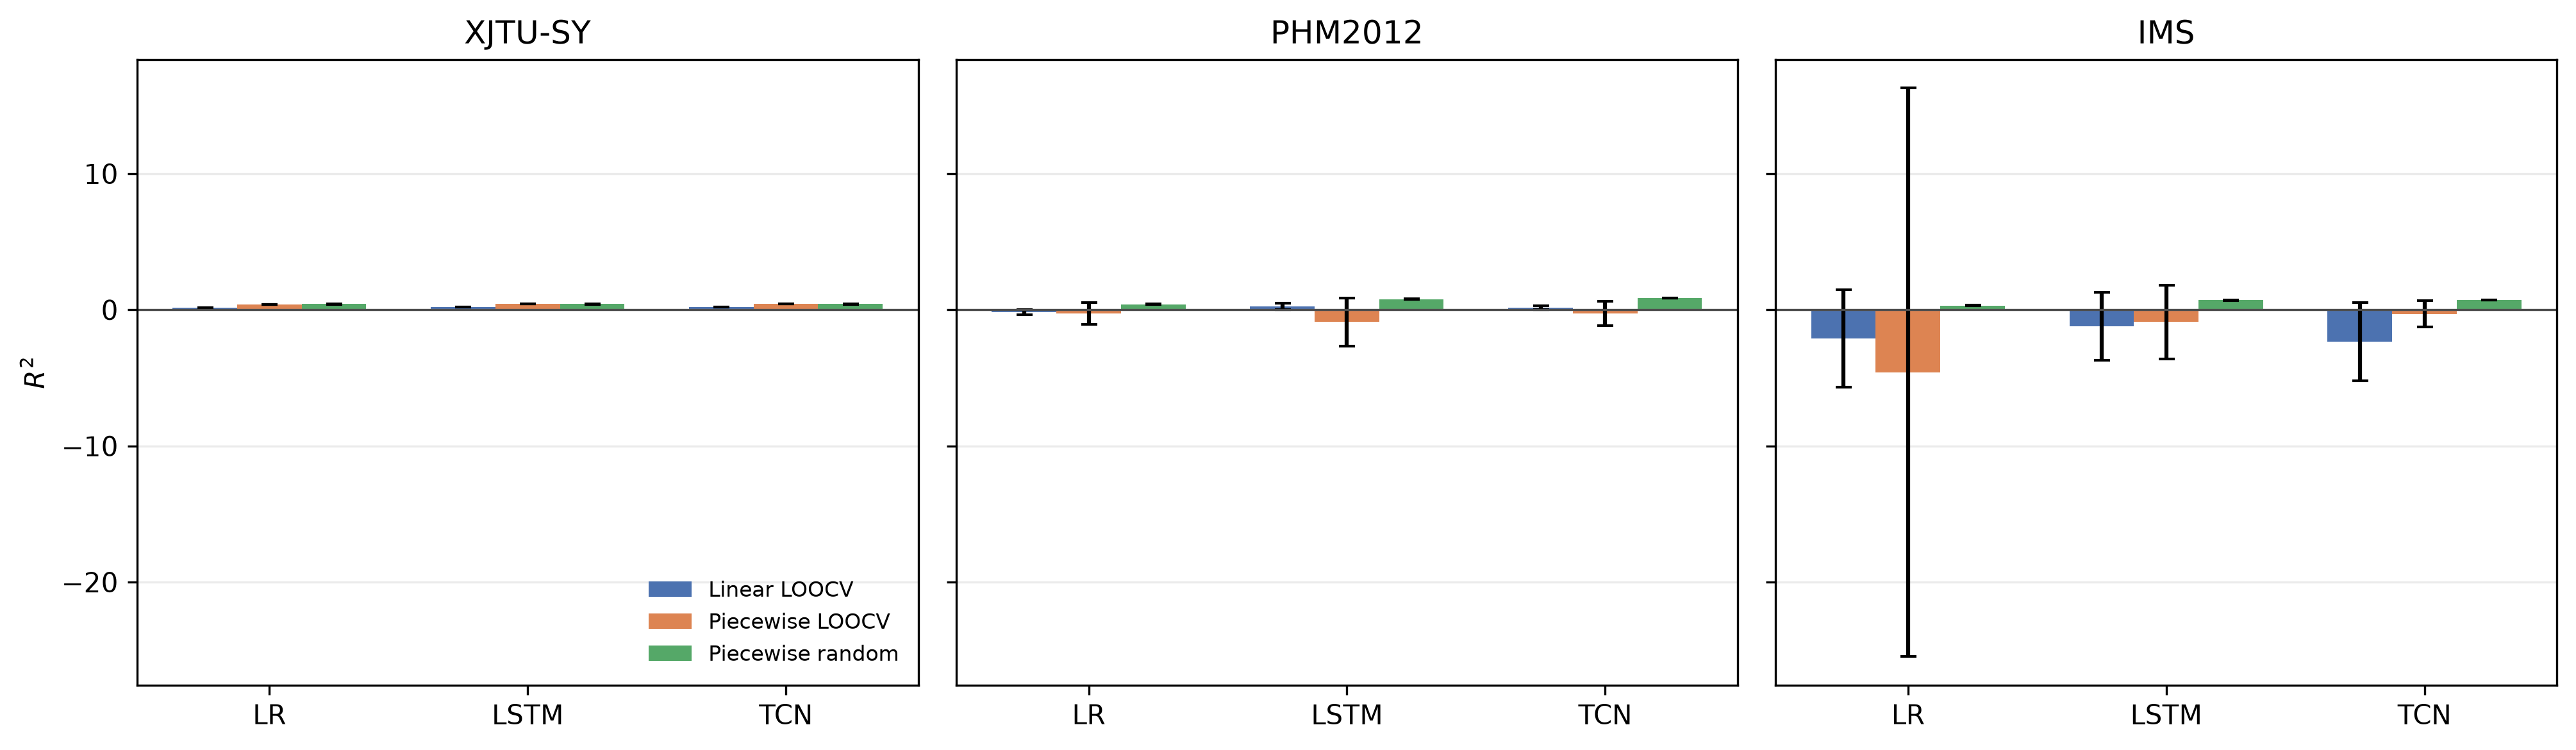
\includegraphics[width=0.48\textwidth]{figures/converged_r2_comparison.png}
\caption{Random time-step splitting consistently raises $R^2$ above linear-LOOCV results, especially on PHM2012 and IMS. Error bars show 95\% confidence intervals for LOOCV and observed min--max ranges for random splits.}
\label{fig:r2}
\end{figure}

\subsection{Constant Baseline and Cross-Bearing Generalization}
The constant predictor has $R^2 \approx 0.000$ on every dataset and label family. Several linear-LOOCV results are below this floor, especially on IMS, where a model must extrapolate across different test rigs and fault modes. This is not a numerical artifact: it shows that cross-bearing generalization is the real challenge. Random time-step splitting hides this failure because test windows come from the same bearings and nearby temporal positions as training windows.

\subsection{Split Sensitivity Results}
Table~\ref{tab:sensitivity} reports TCN results under piecewise labels for the two additional random ratios and the chronological time-block split. The random-ratio results are stable: 60/20/20 and 80/10/10 both remain high, in the same range as the main 70/15/15 result. In contrast, chronological time-block splitting produces large negative $R^2$ on all three datasets. The contrast indicates that the random-split effect is not an artifact of one particular random ratio; it is consistent with within-trajectory interpolation. The negative chronological results should not be read as a pure leakage effect because temporal extrapolation and degradation-stage imbalance also contribute.

\begin{table}[t]
\centering
\caption{TCN split sensitivity with piecewise labels. Random rows are mean [min--max] over seeds 42, 43, 44; time-block uses chronological 70/15/15 per bearing.}
\label{tab:sensitivity}
\small
\begin{tabular}{llc}
\toprule
Dataset & Split & $R^2$ \\
\midrule
XJTU-SY & Random 60/20/20 & 0.422 [0.400; 0.436] \\
 & Random 80/10/10 & 0.439 [0.410; 0.458] \\
 & Time-block 70/15/15 & $-4.957$ \\
\midrule
PHM2012 & Random 60/20/20 & 0.857 [0.847; 0.863] \\
 & Random 80/10/10 & 0.879 [0.872; 0.885] \\
 & Time-block 70/15/15 & $-1.812$ \\
\midrule
IMS & Random 60/20/20 & 0.703 [0.698; 0.708] \\
 & Random 80/10/10 & 0.720 [0.716; 0.727] \\
 & Time-block 70/15/15 & $-7.991$ \\
\bottomrule
\end{tabular}
\end{table}


\subsection{Normalization Sensitivity}
The main results normalize RUL within each trajectory, which assumes end-of-life information when constructing the target. To test the sensitivity of this choice, we constructed global-normalized labels for PHM2012 using a common maximum across all trajectories and repeated the TCN comparison. PHM2012 was selected for this sensitivity analysis because its six trajectories exhibit relatively larger differences in normalized lifetime proportions, making it a more sensitive case for examining the effect of normalization strategy. For linear labels, global normalization reduces linear-LOOCV $R^2$ from $0.174$ to $-5.912$ on PHM2012, while piecewise random splitting remains high ($0.904$ across three seeds). For piecewise labels, global normalization leaves the LOOCV result similar ($-0.263$ versus $-0.260$) and random splitting at $0.859$. This confirms that per-trajectory normalization is not the main driver of the random-split optimism, but it can materially change the difficulty of cross-bearing linear-RUL evaluation. A deployment-oriented protocol should therefore state which target normalization is used. Extending this control to all datasets is future work.

\subsection{Validation-Bearing Sensitivity}
LOOCV also depends on which bearing is selected for validation. We repeated PHM2012 TCN linear-LOOCV with validation bearings shifted by one, two, and three positions. The mean linear-LOOCV $R^2$ changed from $0.089$ to $0.191$ to $0.262$ across the three validation rotations, with fold-level variability remaining high. This shows that validation-bearing selection contributes to fold-level variability and should be disclosed or varied in future benchmarks; the main conclusion that random splitting substantially exceeds cross-bearing LOOCV is unchanged across all rotations. These runs are independent deep-learning repetitions, so the exact offset-1 mean differs from the main-table run; the analysis is intended to test the stability and direction of the validation-bearing effect rather than to reproduce the main table exactly.

\subsection{Protocol-Induced Differences and Their Boundary}
We evaluated the protocol family often used in recent bearing RUL benchmarks: piecewise 80\% plateau labels, random time-step splitting, converged deep training, and standard statistical features. Under this protocol, deep models reach $R^2$ values of $0.70$--$0.86$ on PHM2012 and IMS, substantially above the linear-LOOCV values.

We do not reproduce $R^2>0.99$. The accurate statement is that protocol-induced differences are reproducible at the protocol level, but the magnitude in our reproduced protocol family does not reach the near-perfect range reported by some papers. Public code and checkpoints were not available in our environment for the cited papers, so exact reproduction is not possible. We therefore do not claim that all published near-perfect values are explained by evaluation design; our results are consistent with the view that within-trajectory dependence and interpolation can make estimates optimistic.

\section{Discussion}
\subsection{Random Splitting Measures Within-Trajectory Interpolation}
We distinguish tracking a known bearing, where interpolation-friendly evaluation can be useful, from first diagnosis of a new asset, where a stricter proxy for unseen-bearing generalization under the available benchmark data is the relevant evidence. Sliding windows from one bearing are strongly autocorrelated. A random split places test windows from the same trajectory in the training set, so the model can interpolate across almost identical operating phases. Under LOOCV, the test bearing is completely absent during training. The large gaps on PHM2012 and IMS show that the problem is primarily within-trajectory interpolation relative to the intended cross-bearing prediction task, rather than model capacity.

\subsection{Cross-Bearing LOOCV Provides a Stricter Proxy for Unseen-Bearing Generalization}
In LOOCV, the held-out test bearing is absent from both training and validation. The protocol therefore answers a different question from random splitting: whether a model can generalize to a bearing whose trajectory has not been observed. Several linear-LOOCV results fall below the constant baseline, especially on IMS. That is not a numerical artifact. It means the model is sometimes worse than predicting the mean when it must leave the training trajectory.

\subsection{Chronological Splitting Measures Temporal Extrapolation}
Chronological splitting keeps the test bearing in training but evaluates later stages of the same trajectory. The negative $R^2$ values in Table~\ref{tab:sensitivity} reflect temporal extrapolation and degradation-stage imbalance as well as the absence of random interleaving. The comparison is still useful because it shows that random splitting, not chronological ordering, is what raises the scores on the same data.

Piecewise labels matter for a second reason: the 80\% plateau makes the label almost constant for most of life. On XJTU-SY, this improves apparent regression performance because the model only needs to recognize the transition region. On PHM2012 and IMS, the plateau can also interact with distribution shift and produce poor LOOCV results. The two practices should be reported separately, not combined into a single optimistic-bias multiplier.
\subsection{Label Construction Changes Target Difficulty}

Although $R^2$ reflects explained variance, MAE and RMSE quantify absolute prediction deviations. Table~\ref{tab:errors} confirms that the protocol effect is not an artifact of the $R^2$ scale: the piecewise-random protocol consistently reduces RMSE and MAE relative to the linear-LOOCV protocol across all three datasets.

\subsection{Implications for Bearing RUL Benchmarks}
For benchmark reporting, $R^2$ values are not comparable unless the split and label protocols are specified. The complete $2 \times 2$ design in Table~\ref{tab:factorial} separates label, split, and interaction effects more cleanly than a single protocol comparison. MAE and RMSE should accompany $R^2$; a negative $R^2$ under distribution shift can otherwise obscure whether absolute error is actually large.

\subsection{Implications for Predictive Maintenance Deployment}
Benchmark scores are often used to assess deployment readiness, select models, set intervention thresholds, and plan maintenance windows. If the evaluation protocol permits within-trajectory interpolation, a high score may not transfer to a new asset or a changed operating condition. This can lead to overconfident deployment, inappropriate maintenance timing, or excessive intervention. The STAR template therefore treats evaluation protocol as part of deployment-reliability assessment, not as a purely methodological detail.

For example, an enterprise selecting a model for a new production line may rely on a random-split benchmark and choose a model with a high reported $R^2$; under cross-bearing LOOCV on the same public data, the same model can fall below the constant baseline. Maintenance intervals planned from the optimistic score could lead to inappropriate maintenance timing, such as interventions scheduled too late or too early, and may contribute to unplanned downtime, spare-parts inventory pressure, or intervention cost. In manufacturing practice, the directly evaluated scenario is commissioning or monitoring a new bearing whose trajectory was not part of the training population. Changed operating conditions and machine-station transfer are not directly tested here. A random-split score answers whether the model can interpolate the already observed degradation of the same bearings; a cross-bearing score answers whether the model can support decisions before the new asset has accumulated a long history. STAR therefore provides a practical way to distinguish these two use cases during model selection and deployment review.

Table~\ref{tab:deployment_selection} illustrates the model-selection consequence with actual results from this study. Under a random-split benchmark, the best PHM2012 model would be TCN or PatchTST with $R^2$ around $0.85$--$0.86$; under linear LOOCV, PatchTST retains positive performance while TCN drops sharply. On IMS, random-split scores remain positive while linear LOOCV is negative for every model. A deployment-oriented evaluation therefore changes both the selected model and the expected maintenance timing.


\begin{table}[t]
\centering
\caption{Illustrative protocol-dependent model-selection results from the actual experiments. Random split uses piecewise labels; LOOCV uses linear labels.}
\label{tab:deployment_selection}
\small
\begin{tabular}{llcc}
\toprule
Dataset & Model & Piecewise random $R^2$ & Linear LOOCV $R^2$ \\
\midrule
PHM2012 & TCN & 0.843 & 0.174 \\
PHM2012 & PatchTST & 0.823 & 0.369 \\
IMS & TCN & 0.710 & $-2.331$ \\
IMS & PatchTST & 0.659 & $-1.058$ \\
\bottomrule
\end{tabular}
\end{table}

\subsection{What Does a High $R^2$ Measure?}
A high $R^2$ under random window splitting may indicate interpolation capability rather than cross-bearing predictive ability. The model can rely on adjacent windows from the same trajectory and on the monotonic structure of the label. That kind of performance is useful for tracking a known degradation process, but it does not show that the model can handle a new bearing, a different sensor position, or a different operating regime.

The distinction is visible in the LOOCV results: several models fall below the constant baseline on IMS, while the same models reach much higher $R^2$ under random splitting.


\subsection{Positioning and Generalizability of the Benchmark Evidence}
The experiments use publicly available accelerated run-to-failure test beds rather than proprietary field data. This scope is deliberate: the study evaluates whether benchmark protocol choices change the reliability estimate under controlled degradation conditions, not whether any specific model reaches a production-grade performance level on a particular factory line. Field deployment introduces additional confounders such as load variation, sensor drift, maintenance history, and incomplete run-to-failure records, so field validation remains future work rather than a claim of this paper. For industrial readers, the practical implication is that a benchmark score without STAR-type protocol evidence is not sufficient to infer new-asset reliability; for reviewers, the checklist provides a low-cost structure for checking the evidence behind a reported score.

\subsection{Practical Reporting Workflow}
A benchmark result is interpretable only when the following items are reported together:
\begin{enumerate}
    \item the intended task, either unseen-bearing generalization under the benchmark data or trajectory tracking;
    \item the split protocol, including whether the test bearing is present in training;
    \item the label construction and all plateau parameters;
    \item the constant or median predictor baseline; and
    \item per-fold results with CI, RMSE, and MAE in addition to $R^2$.
\end{enumerate}
The STAR template in the next subsection turns these items into a reusable reporting checklist.

\subsection{STAR Reporting Template}
We summarize the experimentally supported reporting choices into the STAR template, which stands for Split integrity, Target integrity, Anchor baseline, and Reporting completeness. In this paper these map to:
\begin{enumerate}
    \item \textbf{Continuous labels}: linear or physics-guided labels as the primary target; plateau parameters should be justified if retained.
    \item \textbf{Leave-one-bearing-out cross-validation}: no training window from the test bearing, with per-fold reporting.
    \item \textbf{Constant predictor baseline}: report the floor below which a model is not informative.
    \item \textbf{Multi-model reporting}: at least two complementary model classes so conclusions are not architecture-specific.
\end{enumerate}
An adaptive debiased label that shortens the plateau and smooths the transition remains a practical intermediate option for applications that need early-stage noise suppression. The current experiments suggest that fixing the split protocol is at least as important as fixing the label.

Table~\ref{tab:star} summarizes the template as a reporting checklist. The checklist is derived from the protocol differences and controls observed in this study rather than from generic best-practice recommendations. STAR is a reporting template, not a scoring or certification system; it specifies a recommended reporting structure for deployment-oriented cross-bearing evaluation rather than an exhaustive reliability certification procedure. Appendix A applies the checklist to representative studies as illustrative reporting extraction; the purpose is to make reporting choices explicit, not to judge the validity of individual models or results.

\begin{table*}[t]
\centering
\caption{STAR reporting structure recommended for deployment-oriented cross-bearing evaluation.}
\label{tab:star}
\small
\resizebox{\textwidth}{!}{%
\begin{tabular}{lll}
\toprule
Component & Recommended cross-bearing reporting practice & Status in this study \\
\midrule
Split integrity & Test bearing absent from training and validation & Random window split does not satisfy; LOOCV satisfies \\
Target integrity & Continuous or explicitly justified label construction & Linear and piecewise labels compared separately \\
Anchor baseline & Constant predictor reported as floor & Included \\
Reporting completeness & Per-fold results, CI, RMSE, MAE, seeds & Included \\
\bottomrule
\end{tabular}}
\end{table*}

Table~\ref{tab:star_before_after} shows the contrast between conventional reporting patterns and the STAR recommendations. The comparison makes the template actionable: a reader can check each row against a submitted benchmark and see which part of the evaluation protocol is missing.

Uncertainty-aware reporting is a direct extension of the STAR checklist. Conformal prediction and quantile-regression methods \cite{mst2024cqr,icsrs2023splitconformal,phme2026conformal,eaai2025explainable} can provide prediction intervals, coverage, and calibration metrics, but these measures are interpretable only when computed under the same split and label constraints as point forecasts. STAR can therefore treat interval coverage, interval width, calibration, and transfer-condition disclosure as part of Reporting completeness, and recommend that the test-bearing information constraints remain unchanged. This study deliberately keeps the primary analysis on point forecasts because the protocol effects are already strong and statistically separable; extending the same factorial decomposition to interval predictors, transfer-learning settings, and field datasets is a natural next step rather than a claim of the present experiments.

\begin{table*}[t]
\centering
\caption{Conventional reporting patterns versus STAR recommendations.}
\label{tab:star_before_after}
\small
\resizebox{\textwidth}{!}{%
\begin{tabular}{lll}
\toprule
Aspect & Conventional pattern & STAR recommendation \\
\midrule
Split & Random window split & Test bearing absent from training and validation \\
Target & Piecewise plateau without justification & Continuous or explicitly justified label \\
Baseline & Constant predictor often omitted & Constant predictor reported \\
Reporting & Final $R^2$ only & Per-fold, CI, RMSE, MAE, seeds \\
\bottomrule
\end{tabular}}
\end{table*}

\subsection{Limitations}
This is a laboratory benchmark methodology study based on public accelerated-life datasets; it does not include field data. We did not reproduce exact published checkpoints because public code was unavailable. IMS has only three held-out test sets, so its confidence intervals are wide; we therefore treat IMS as directional evidence. The external datasets use the same statistical feature pipeline rather than each paper's raw-signal preprocessing. PU is not used because it does not provide run-to-failure trajectories. Trajectory-specific RUL normalization is an offline benchmark construction assumption and should not be interpreted as an online deployment procedure. We do not claim a quantitative prevalence survey; the conclusions concern a commonly used protocol family rather than an assessment of individual papers. Appendix A demonstrates how the STAR checklist can support transparent reporting extraction. Future work should run exact published pipelines when code becomes available and extend STAR to raw-signal models, uncertainty-aware interval predictors, transfer-learning settings, and field datasets when they can be shared.

\section{Conclusion}
Using converged training on XJTU-SY, PHM2012, and IMS, we show that piecewise labels and random time-step splitting consistently produce higher $R^2$ than linear-label LOOCV, with complete separation between protocol groups (Cliff's delta $=1.0$) in all twelve model-dataset cells. These protocol-induced differences are reproducible within our protocol family but do not reach or explain published near-perfect values; exact reproduction of original pipelines remains necessary. The STAR reporting template provides a recommended reporting structure for deployment-oriented cross-bearing evaluation, supporting model selection and review. The contribution is not a new architecture or a generic warning against shuffling time series; it is a controlled quantification of a bearing-RUL-specific interaction between plateau labels and split protocols, whose direction varies across datasets.

\appendix
\section{Illustrative Examples of Reporting Extraction}
To support transparent reporting without judging individual studies, the STAR checklist can be recorded as \emph{reported}, \emph{unclear}, or \emph{unavailable}. \emph{Reported} means that the item is explicitly described in the examined full text; \emph{unclear} means that the description is incomplete or ambiguous; \emph{unavailable} means that the information could not be verified from the examined source. The purpose is to make reporting choices visible, not to classify studies as valid or invalid.

Table~\ref{tab:star_audit} illustrates how reporting choices can be extracted from five examples whose full texts are publicly available from their journals. The coding sheet uses the same three-level vocabulary for candidate studies; rows should be completed only after full-text examination.

\begin{table*}[t]
\centering
\caption{Illustrative examples of reporting extraction. Entries record what can be verified from the examined full texts and are not correctness judgments.}
\label{tab:star_audit}
\small
\resizebox{\textwidth}{!}{%
\begin{tabular}{llllll}
\toprule
Study & Dataset & Split & Target construction & Anchor baseline & Reporting completeness \\
\midrule
Wu and Zhang \cite{wu2020cascade} & PHM2012 & Leave-one-bearing-out & Linear reliability rate & Unavailable & Unavailable \\
Yang et al. \cite{yang2024cnnvaembilstm} & Industrial weaving-machine case & Bearing-level 70/30 train/test & Normalized RUL (construction details unclear) & Unavailable & Data not public; no code \\
Wen et al. \cite{wen2024envelope} & XJTU-SY & Leave-one-bearing-out within condition & Piecewise linear RUL (plateau unclear) & Unavailable & Dataset available; no code \\
Li et al. \cite{li2022twostage} & PHM2012 & Cross-condition bearing holdout & Health percentage after IF (pre-IF plateau) & Unavailable & Data on request; no code \\
Li et al. \cite{li2022soasvm} & IMS & Within-trajectory parity 1:1 & PCA degradation index & Unavailable & Data in article; no code \\
\bottomrule
\end{tabular}}
\end{table*}

\backmatter

\bmhead{Supplementary information}
Supplementary material includes preprocessing scripts, converged training and split sensitivity runners, per-fold and per-seed JSON results, table/figure generators, and additional protocol details.

\clearpage
\section{Per-Fold and Per-Seed Evidence}
\begin{table*}[!ht]
\centering
\caption{Per-fold and per-seed evidence for the protocol effect. LOOCV range is the min--max of linear-label fold $R^2$; seed columns are piecewise-label random-split $R^2$ for seeds 42--49.}
\label{tab:perfold}
\small
\resizebox{\textwidth}{!}{%
\begin{tabular}{lllccccccccc}
\toprule
Dataset & Model & Linear LOOCV range & S42 & S43 & S44 & S45 & S46 & S47 & S48 & S49 & Protocol gap \\
\midrule
XJTU-SY & LinearRegression & 0.176--0.181 & 0.447 & 0.414 & 0.429 & 0.364 & 0.400 & 0.416 & 0.399 & 0.375 & 0.228 \\
XJTU-SY & StatLSTM & 0.220--0.225 & 0.435 & 0.430 & 0.401 & 0.386 & 0.432 & 0.415 & 0.385 & 0.399 & 0.188 \\
XJTU-SY & TCN & 0.219--0.226 & 0.433 & 0.433 & 0.396 & 0.386 & 0.440 & 0.409 & 0.382 & 0.398 & 0.188 \\
XJTU-SY & PatchTST & 0.220--0.226 & 0.453 & 0.425 & 0.438 & 0.386 & 0.428 & 0.413 & 0.380 & 0.402 & 0.194 \\
PHM2012 & LinearRegression & -0.444--0.101 & 0.376 & 0.396 & 0.420 & 0.435 & 0.426 & 0.465 & 0.424 & 0.385 & 0.584 \\
PHM2012 & StatLSTM & -0.057--0.514 & 0.778 & 0.803 & 0.791 & 0.809 & 0.801 & 0.762 & 0.776 & 0.757 & 0.540 \\
PHM2012 & TCN & 0.033--0.341 & 0.865 & 0.859 & 0.862 & 0.845 & 0.844 & 0.827 & 0.818 & 0.821 & 0.669 \\
PHM2012 & PatchTST & 0.135--0.657 & 0.841 & 0.854 & 0.855 & 0.817 & 0.857 & 0.775 & 0.808 & 0.776 & 0.454 \\
IMS & LinearRegression & $-3.000$ to $-0.452$ & 0.328 & 0.313 & 0.318 & 0.333 & 0.315 & 0.310 & 0.327 & 0.319 & 2.429 \\
IMS & StatLSTM & $-2.372$ to $-0.592$ & 0.706 & 0.695 & 0.697 & 0.691 & 0.688 & 0.684 & 0.681 & 0.694 & 1.900 \\
IMS & TCN & $-3.013$ to $-0.990$ & 0.714 & 0.715 & 0.717 & 0.706 & 0.706 & 0.710 & 0.703 & 0.712 & 3.041 \\
IMS & PatchTST & $-1.683$ to $-0.114$ & 0.674 & 0.689 & 0.679 & 0.651 & 0.639 & 0.647 & 0.643 & 0.653 & 1.718 \\
\bottomrule
\end{tabular}}
\end{table*}

The main-table LOOCV runs use the designated fixed validation-bearing offset. The validation-bearing sensitivity runs reported in the text are independent deep-learning repetitions from \texttt{validation\_sensitivity\_phm\_tcn.json}; their offset-1 mean is therefore a stability check rather than a reproduction of the main-table run.


\section*{Declarations}
\begin{itemize}
\item Funding: This research received no specific grant from any funding agency in the public, commercial, or not-for-profit sectors.
\item Conflict of interest: The authors declare that they have no known competing financial interests or personal relationships that could have appeared to influence the work reported in this paper.
\item Ethics approval and consent to participate: Not applicable.
\item Consent for publication: Not applicable.
\item Data availability: The XJTU-SY, PHM2012, and IMS datasets are publicly available from their original sources.
\item Code availability: The reproducibility package is available at \url{https://github.com/KKK-cell441/rul-evaluation-star} and archived at \url{https://doi.org/10.5281/zenodo.21887653}.
\item Author contribution: Zhongkuan Ma: Conceptualization, Methodology, Software, Validation, Formal analysis, Writing - Original Draft, Writing - Review \& Editing.
\item ORCID: 0009-0003-4491-6619.
\end{itemize}

\begin{thebibliography}{99}

\bibitem{lei2018machinery}
Y. Lei, N. Li, L. Guo, N. Li, T. Yan, and J. Lin,
``Machinery health prognostics: A systematic review from data acquisition to RUL prediction,''
\textit{Mech. Syst. Signal Process.}, vol.~104, pp.~799--834, 2018.

\bibitem{zhao2019deep}
R. Zhao, R. Yan, Z. Chen, K. Mao, P. Wang, and R. X. Gao,
``Deep learning and its applications to machine health monitoring,''
\textit{Mech. Syst. Signal Process.}, vol.~115, pp.~213--237, 2019.

\bibitem{rul_lstm_uq_2022}
J. Yang, Y. Peng, J. Xie, and P. Wang,
``Remaining useful life prediction method for bearings based on LSTM with uncertainty quantification,''
\textit{Sensors}, vol.~22, no.~12, p.~4549, 2022. doi:10.3390/s22124549.

\bibitem{reg_lstm_2021}
Z.-H. Liu, X.-D. Meng, H.-L. Wei, L. Chen, B.-L. Lu, Z.-H. Wang, and L. Chen,
``A regularized LSTM method for predicting remaining useful life of rolling bearings,''
\textit{Int. J. Autom. Comput.}, vol.~18, no.~4, pp.~581--593, 2021. doi:10.1007/s11633-020-1276-6.

\bibitem{gru_tim_2021}
Z. Que, X. Jin, and Z. Xu,
``Remaining useful life prediction for bearings based on a gated recurrent unit,''
\textit{IEEE Trans. Instrum. Meas.}, vol.~70, pp.~1--11, 2021. doi:10.1109/tim.2021.3054025.

\bibitem{wu2020cascade}
Q. Wu and C. Zhang,
``Cascade fusion convolutional long-short time memory network for remaining useful life prediction of rolling bearing,''
\textit{IEEE Access}, vol.~8, pp.~32957--32965, 2020. doi:10.1109/access.2020.2970444.

\bibitem{yang2024cnnvaembilstm}
L. Yang, Y. Jiang, K. Zeng, and T. Peng,
``Rolling bearing remaining useful life prediction based on CNN-VAE-MBiLSTM,''
\textit{Sensors}, vol.~24, no.~10, p.~2992, 2024. doi:10.3390/s24102992.

\bibitem{wen2024envelope}
H. Wen, L. Zhang, and J. K. Sinha,
``From envelope spectra to bearing remaining useful life: An intelligent vibration-based prediction model with quantified uncertainty,''
\textit{Sensors}, vol.~24, no.~22, p.~7257, 2024. doi:10.3390/s24227257.

\bibitem{li2022twostage}
X. Li, K. Zhang, W. Li, Y. Feng, and R. Liu,
``A two-stage transfer regression convolutional neural network for bearing remaining useful life prediction,''
\textit{Machines}, vol.~10, no.~5, p.~369, 2022. doi:10.3390/machines10050369.

\bibitem{li2022soasvm}
X. Li, S. An, Y. Shi, and Y. Huang,
``Remaining useful life estimation of rolling bearing based on SOA-SVM algorithm,''
\textit{Machines}, vol.~10, no.~9, p.~729, 2022. doi:10.3390/machines10090729.

\bibitem{transformer_tim_2023}
H. Peng, B. Jiang, Z. Mao, and S. Liu,
``Local enhancing transformer with temporal convolutional attention mechanism for bearings remaining useful life prediction,''
\textit{IEEE Trans. Instrum. Meas.}, vol.~72, pp.~1--12, 2023. doi:10.1109/tim.2023.3291787.

\bibitem{zhao2021deep}
M. Zhao, M. Kang, B. Tang, and M. Pecht,
``Deep learning for bearing prognostics: A comprehensive review,''
\textit{IEEE Trans. Rel.}, vol.~70, no.~4, pp.~1431--1451, 2021.

\bibitem{caesarendra2021machine}
W. Caesarendra and T. Tjahjowidodo,
``Machine learning methods for bearing fault diagnosis: A comprehensive review,''
\textit{Mech. Syst. Signal Process.}, vol.~152, p.~107397, 2021.

\bibitem{li2022physics}
T. Li, Z. Zhou, S. Li, and Y. Chen,
``Physics-informed neural networks for bearing remaining useful life prediction,''
\textit{Reliab. Eng. Syst. Saf.}, vol.~224, p.~108548, 2022.

\bibitem{ince2016real}
T. Ince, S. Kiranyaz, L. Eren, M. Askar, and M. Gabbouj,
``Real-time motor fault detection by 1-D convolutional neural networks,''
\textit{IEEE Trans. Ind. Electron.}, vol.~63, no.~11, pp.~7067--7075, 2016.

\bibitem{vaswani2017attention}
A. Vaswani, N. Shazeer, N. Parmar, J. Uszkoreit, L. Jones, A. N. Gomez, L. Kaiser, and I. Polosukhin,
``Attention is all you need,''
in \textit{Proc. NeurIPS}, vol.~30, 2017.

\bibitem{paris1963critical}
P. Paris and F. Erdogan,
``A critical analysis of crack propagation laws,''
\textit{J. Basic Eng.}, vol.~85, no.~4, pp.~528--534, 1963.

\bibitem{kotzalas2004fatigue}
M. N. Kotzalas and T. A. Harris,
``Fatigue failure and life prediction of rolling bearings,''
\textit{Tribol. Trans.}, vol.~47, no.~3, pp.~409--418, 2004.

\bibitem{xjtusy2019dataset}
B. Wang, Y. Lei, N. Li, and N. Li,
``XJTU-SY rolling element bearing accelerated life test dataset,''
\textit{Data in Brief}, vol.~25, p.~104122, 2019.

\bibitem{nectoux2012pronostia}
P. Nectoux, R. Gouriveau, K. Medjaher, E. Ramasso, B. Chebel-Morello, N. Zerhouni, and C. Varnier,
``PRONOSTIA: An experimental platform for bearings accelerated degradation tests,''
in \textit{IEEE Int. Conf. Prognostics and Health Management}, 2012, pp.~1--8.

\bibitem{ims2006}
H. Qiu, J. Lee, J. Lin, and G. Yu,
``Wavelet filter-based weak signature detection method and its application on rolling element bearing prognostics,''
\textit{J. Sound Vib.}, vol.~289, no.~4--5, pp.~1066--1090, 2006.

\bibitem{leakage_nature}
N. G. Davies et al.,
``Data leakage jeopardizes ecological applications of machine learning,''
\textit{Nat. Ecol. Evol.}, vol.~7, 2023.

\bibitem{leakage_frontiers}
J. A. Long, J. F. Levesque, and D. L. Huffman,
``Bursting the bubble: Data leakage and inflated deep learning accuracy in multivariate time-series frailty classification,''
\textit{Front. Comput. Sci.}, vol.~8, 2026. doi:10.3389/fcomp.2026.1700489.
\bibitem{patchtst2023}
Y. Nie, N. H. Nguyen, P. Sinthong, and J. Kalagnanam,
``A time series is worth 64 words: Long-term forecasting with transformers,''
in \textit{Proc. Int. Conf. Learn. Represent.}, 2023.


\bibitem{phmconf2025rethinking}
M. Salinas-Camus, K. Goebel, and N. Eleftheroglou,
``Rethinking RUL prediction,'' in \textit{Annu. Conf. PHM Soc.}, vol.~17, 2025. doi:10.36001/phmconf.2025.v17i1.4361.

\bibitem{review2020bearing}
Z. Xia, Q. Guan, Y. Gao, X. Chen, and X. Zhai,
``Review on remaining useful life prediction methods of bearing,'' in \textit{Int. Conf. Prognostics and System Health Management}, 2020. doi:10.1109/PHM-Jinan48558.2020.00083.

\bibitem{mst2024cqr}
S. Mao, X. Li, and B. Zhao,
``Remaining useful life prediction based on time-series features and conformalized quantile regression,'' \textit{Meas. Sci. Technol.}, vol.~35, 2024. doi:10.1088/1361-6501/ad762c.

\bibitem{icsrs2023splitconformal}
W. Xu and E. Zio,
``A general data-driven framework for remaining useful life estimation with uncertainty quantification using split conformal prediction,'' in \textit{Int. Conf. Syst. Reliab. Saf.}, 2023. doi:10.1109/ICSRS59833.2023.10381131.

\bibitem{phme2026conformal}
S. Wang, Y. Vidal, and F. Pozo,
``Uncertainty-aware bearing remaining useful life prediction based on conformal prediction,'' in \textit{PHM Soc. Eur. Conf.}, vol.~9, 2026. doi:10.36001/phme.2026.v9i1.4902.

\bibitem{ress2022bayesian}
R. Zhu, Y. Chen, W. Peng, and Z.-S. Ye,
``Bayesian deep-learning for RUL prediction: An active learning perspective,'' \textit{Reliab. Eng. Syst. Saf.}, vol.~228, 2022. doi:10.1016/j.ress.2022.108758.

\bibitem{eaai2025explainable}
T. Zhang and H. Wang,
``Explainable remaining useful life uncertainty prediction method for rolling bearing,'' \textit{Eng. Appl. Artif. Intell.}, vol.~142, 2025. doi:10.1016/j.engappai.2025.112114.
\end{thebibliography}

\end{document}
